\documentclass[10pt,letterpaper]{article}
\usepackage[top=0.85in,left=2.75in,footskip=0.75in]{geometry}

% Use adjustwidth environment to exceed column width (see example table in text)
\usepackage{changepage}

% Use Unicode characters when possible
\usepackage[utf8]{inputenc}

% textcomp package and marvosym package for additional characters
\usepackage{textcomp,marvosym}

% fixltx2e package for \textsubscript
\usepackage{fixltx2e}

% amsmath and amssymb packages, useful for mathematical formulas and symbols
\usepackage{amsmath,amssymb}

% Use nameref to cite supporting information files (see Supporting Information section for more info)
\usepackage{nameref,hyperref}

% line numbers
\usepackage[right]{lineno}

% ligatures disabled
\usepackage{microtype}
\DisableLigatures[f]{encoding = *, family = * }

% rotating package for sideways tables
\usepackage{rotating}

% Remove comment for double spacing
\usepackage{setspace} 
\doublespacing

% Text layout
\raggedright
\setlength{\parindent}{0.5cm}
\textwidth 5.25in 
\textheight 8.75in

% Bold the 'Figure #' in the caption and separate it from the title/caption with a period
% Captions will be left justified
\usepackage[aboveskip=1pt,labelfont=bf,labelsep=period,justification=raggedright,singlelinecheck=off]{caption}

% Remove brackets from numbering in List of References
\makeatletter
\renewcommand{\@biblabel}[1]{\quad#1.}
\makeatother

% Leave date blank
\date{}

% Header and Footer with logo
\usepackage{lastpage,fancyhdr,graphicx}
\usepackage{epstopdf}
\pagestyle{myheadings}
\pagestyle{fancy}
\fancyhf{}
\lhead{
\includegraphics[width=2.0in]{PLOS-submission.eps}}
\rfoot{\thepage/\pageref{LastPage}}
\renewcommand{\footrule}{\hrule height 2pt \vspace{2mm}}
\fancyheadoffset[L]{2.25in}
\fancyfootoffset[L]{2.25in}
\lfoot{\sf PLOS}

%% Include all macros below

\newcommand{\lorem}{{\bf LOREM}}
\newcommand{\ipsum}{{\bf IPSUM}}

%% END MACROS SECTION


%%% Begin BWP
%\usepackage{amsmath, amsthm, amssymb, wasysym, graphicx}
%\usepackage[small, hang, bf]{caption}


%% CHOOSE!  Use PLOS idiot-biologist-content-free style, or
%% informative style for internal use?
% cite package, to clean up citations in the main text. Do not remove.
\usepackage{cite}
% Use the PLoS provided BiBTeX style
\bibliographystyle{plos2015}
\usepackage[normalem]{ulem}
%\usepackage{natbib}
%\bibstyle{plainnat}
%\renewcommand\cite{\citep}
%\newcommand\citepossessive[1]{\citeauthor{#1}'s \citeyearpar{#1}}

%\usepackage{polski} % For one dude's name in one bibliography entry!
%\usepackage[utf8]{inputenc}
%\a[lf]{berenis}
%\usepackage[LY1]{fontenc}

\usepackage{algorithm2e}

\newcommand\eq[1]{Eq.~\ref{#1}}
\newcommand\fig[1]{Fig.~\ref{#1}}
\newcommand\sref[1]{Section~\ref{#1}}
\let\oldmarginpar\marginpar
\renewcommand{\marginpar}[1]{\oldmarginpar{\linespread{1}\scriptsize{#1}}}

% PLOS wants \paragraph for some reason... or do they...!?
%\renewcommand{\subsubsection}[1]{\paragraph{#1}}

\setlength{\marginparwidth}{55mm}


\newcommand\argmin{\mathop{\mbox{{\rm argmin}}}\limits}
\newcommand{\noprint}[1]{}

%%% End BWP


\begin{document}
\vspace*{0.35in}

% Title must be 250 characters or less.
% Please capitalize all terms in the title except conjunctions, prepositions, and articles.
\begin{flushleft}
{\Large
  \textbf\newline{A Multi-Channel Electrode for Chronic Recording and Safe Current-Steered Stimulation}
}
\newline
% Insert author names, affiliations and corresponding author email (do not include titles, positions, or degrees).
\\
Ben Pearre\textsuperscript{1,a,\textcurrency},
Sanne~Moorman\textsuperscript{1,b},
Jun Shen\textsuperscript{1,c},
Stuart F.~Cogan\textsuperscript{2,d}
Timothy J.~Gardner\textsuperscript{1,e}
\\
\bigskip
\textsuperscript{1} Department of Biology, Boston University, Boston, Massachusetts, United States of America\\
\textsuperscript{2} Department of Bioengineering, University of Texas, Dallas, Texas, United States of America
\\
\bigskip

% Insert additional author notes using the symbols described below. Insert symbol callouts after author names as necessary.
% 
% Remove or comment out the author notes below if they aren't used.
%
% Primary Equal Contribution Note
%\Yinyang These authors contributed equally to this work.
Author \textsuperscript{a}~did something, we think.  The histology data analysis was by Author \textsuperscript{b}. Author \textsuperscript{c} performed all surgeries.  Authors \textsuperscript{b} and \textsuperscript{c} did the histologies.  Author \textsuperscript{d} developed the iridium oxide coating technique.  Author \textsuperscript{e}, the PI, designed and guided the experiment and this paper.

% Additional Equal Contribution Note
% Also use this double-dagger symbol for special authorship notes, such as senior authorship.
%\ddag These authors also contributed equally to this work.

% Current address notes
%\textcurrency a Insert current address of first author with an address update
% \textcurrency b Insert current address of second author with an address update
% \textcurrency c Insert current address of third author with an address update

% Deceased author note
%\dag Deceased

% Group/Consortium Author Note
%\textpilcrow Membership list can be found in the Acknowledgments section.

% Use the asterisk to denote corresponding authorship and provide email address in note below.
\textsuperscript{\textcurrency} Corresponding author: bwpearre@gmail.com (BP)

\end{flushleft}

\reversemarginpar
%%% End PLOS header template


\begin{abstract}

  Electrical control of the brain facilitates a variety of therapeutic
  and scientific goals, from treating sensory, motor, and cognitive
  defects to exploring the effects of disrupting or modifying the
  brain's behaviour in real time.  These methods are limited by the
  brain's immune reaction to foreign matter: over a period of months,
  glia encapsulate the electrodes, isolating them from neurons. Small
  electrodes ($<$ 10 $\mu$m) minimise encapsulation, and thus can both
  record single neurons for many months and precisely stimulate small
  groups of neurons.  However, such small electrodes are deliecate,
  and their high impedance requires stimulation voltages that exceed
  the water hydrolysis point.

  We have previously developed an electrode design in which groups of
  thin electrodes support each other during insertion and then splay
  in the brain. Here we describe the splaying properties of these
  electrode arrays.  We present preliminary results showing that these
  electrodes remain capable of recording individual spikes for a year
  after implantatiion, and that the spatial scale of the splaying is
  sufficient to allow the steering of current between the
  electrodes. We show a proof of concept of two consequences of
  current steering: it can produce neural responses while keeping
  stimulation voltages below safety limits, and it permits some
  control over the shape of the response.

\end{abstract}

\linenumbers
\section{Introduction}

Direct control of the brain---the ability to sense and modify its
dynamics in real time---is a longstanding goal in neuroscience,
engineering, and medicine. Sensing has been achieved on a variety of
spatial and temporal scales in humans and non-humans, using fMRI,
scalp electrodes, trans-cranial magnetic stimulation,
optigenetics, and with surgically implanted electrodes, both on the
surface of the cortex and implanted into deep brain areas. The gold
standard for spatial and temporal resolution is patch clamping, which
can electrically record individual spikes, but is at present infeasible for
chronic implants in behaving animals. Small extracellular electrodes
can potentially provide high spatial and temporal resolution,
recording individual neurons and stimulating regions on the scale
of a single dendritic tree. Increasing the channel count of these
electrodes allows recording signals from different locations
simultaneously, as well as greater control over
where current is delivered during stimulation. Decreasing the size of the electrodes improves spatial resolution and chronic recording capability, but at the expense of robustness and the ability to inject biologically relevant currents at safe voltages. We propose that a multichannel electrode
arrays consisting of thin carbon fibres, combined with appropriate
current steering, can achieve fine spatial resolution, biological
compatibility, and safe stimulation, and can produce a variety of different
neural dynamics.

Much of the work in current steering in the brain is due to interest
in deep brain stimulation (DBS).  Despite the lack of understanding of
the precise mechanisms of DBS, it has been successfully used to treat
various movement disorders (especially those associated with
Parkinson's disease), epilepsy, Alzheimer's, chronic pain, cluster
headache, depression, OCD, addictive behaviours, anorexia, and others
\cite{Udupa2015dbs}. DBS electrodes usually consist of single rods
1.2--1.6 mm in diameter with 4--32 contacts. Large electrodes cause
significant damage both during and after surgery---over the course of
weeks and months, glia gradually encapsulate intruding electrodes,
rendering them less effective over time. For example,
\cite{Butson2008steering} reports a 500-$\mu$m encapsulation layer for
the $\sim$~1.3-mm electrodes common in DBS.  This encapsulation
results in ever-increasing stimulation thresholds, rendering the
electrodes unable to record as effectively
\cite{Barrese2016electrodestability,Biran2005gliosis,Polikov2005gliosis,Winslow2010gliosis}.

Even before glial encapsulation, large electrodes lack sufficient
spatial resolution to record or stimulate near the single-neuron
spatial scale, and instead can sense and modify only local field
potentials. At this spatial scale, most current-steering methods use
computational models of brain tissue to predict steering
configurations that preferentially target the intended area, or make
up for errors in electrode placement during surgery
\cite{Holloway2005stereotaxy}. One approach
\cite{Butson2008steering,Chaturvedi2012} builds a model of the tissue
of interest using magnetic resonance imaging (MRI) and diffusion
tensor imaging (DTI) \cite{Tuch2001conductivity,Alexander2007dti}.
This produces data with voxels of roughly 2 mm\textsuperscript{3}.
They then use finite element analysis to design current-steering
patterns for the desired target.\marginpar{Lots more references
  might be added here, all of which have spatial resolution on this
  order and a variety of temporal resolutions; choose $\approx$3 or
  just cite a review?} The accuracy of this and related approaches is
appropriate given the size of DBS electrodes; however, the techniques
will not provide sufficient accuracy to take advantage of the control
available with small electrodes.

Steering current allows some degree of delivery of stimulus to
locations between electrodes, allowing control policies to take the
place of electrodes with higher channel count. For example, 64-channel
electrode arrays, with electrode as closely packed as 30 $\mu$m, were
used to stimulate macaque retina {\em in vitro}
\cite{Jepson2014steering_in_retina}. They stimulated the retina using
single electrodes or combinations of three electrodes with
charge-balanced pulses, and found that retinal response could be
predicted with a piecewise linear model of the steered current. The
connectivity of retinal cells differs from that in most brain regions
of interest, but we believe that this experiment nonetheless hints at the
potential of neuron-scale current steering.

Most DBS systems deliver some fixed stimulation pattern continuously.
Recently, interest in using biological feedback to tune medical
devices has grown.  For feedback
control, most systems rely on large-spatial-scale metrics such as local
field potentials (LFP) \cite{Priori2013adbs-lfp} and other macroscopic
measures of outcome such as surface electromyography and accelerations
\cite{Afshar2012closedloop,Basu2013dbsFeedback}\marginpar{Great
  review: \cite{Priori2015review}}. However, neuron-scale electrodes
have shown promise for treatment of Parkinsonian symptoms in
monkeys. A tungsten microelectrode stimulating the globus pallidum in
response to individual spikes detected by a similar electrode in the
related brain area M1 proved more effective than more standard
feedback paradigms or open-loop control \cite{Rosin2011adbs}.

Insults during insertion, glial encapsulation over time, and poor spatial
scale of large electrodes are all mitigated by electrodes $<$ 10
$\mu$m, but these present two difficulties: they are too fragile to
insert easily, and during stimulation, their small surface area
requires dangerously high voltage in order to deliver sufficient
current to induce response.

The electrode array of \cite{Guitchounts2013electrode} overcomes the
structural fragility of thin electrodes by using multiple (in our
case, 16) shanks each of which, at 7 $\mu$m, is small enough to avoid
adverse tissue reactions.  They bundle together to support each other
structurally during implantation, and separate and splay in the brain,
giving randomly distributed sites for recording and stimulation. Here
we quantify that splay.

In a current-controlled stimulating electrode,\marginpar{Why
  current-controlled? E.g. \cite{Chaturvedi2012}?} the voltage
required to induce neural activity goes up as the impedance increases
and charge injection capacity decreases. Stimulation voltage above the
hydrolysis point of water (around 1.3 V) increases the risk of tissue
damage as well as leading to erosion of carbon electrodes due to
oxidative etching \cite{Tamakov2010erosion}. This voltage limit is not
a limiting factor for large DBS electrodes, whose surface area tends
to be ample and which are in any case encapsulated by glia, but it
creates a problem for our small electrodes (in our case the area per
shank is around 2000 $\mu\textrm{m}^2$): their impedance is high and
their charge delivery capacity is poor, leading to high voltage
requirements for stimulation.

We address the voltage problem in two ways. First, we confirm that
electroplating the electrodes in iridium oxide, as suggested by
\cite{Cogan2008electrodes}, \marginpar{Confirm improvement in charge
  delivery. Yarden has numbers of gold $\rightarrow$ IrOx, but do we
  have carbon $\rightarrow$ IrOx anywhere more systematic than my own
  data? But more than that, since we only did this with one chronic
  electrode (and the short-term birds), is it even worth listing here?
  Or should I just mention it in Methods?} leads to roughly a tenfold
improvement in both impedance and charge injection capacity. Second,
we provide evidence that appropriate choice of current-steering
configuration can be used to reduce stimulation voltage.

Due to their size, the multichannel, spatially distributed,
micron-scale arrays introduced in \cite{Guitchounts2013electrode}
allow long-term single-unit recordings, enabling new experiments
investigating how the brain changes on timescales on the order of a year. Here
we provide evidence showing:
\begin{itemize}
\item How often the electrodes splay correctly in the brain, and the spatial scale of that splay.
\item That the electrodes can record activity in single units\marginpar{Is this claim easily justifiable given the unreliability of spike-sorting?} a year after surgery.
\item That the electrodes can be used to stimulate the brain.
\item That the spatial scale of splay is sufficient to allow effective current steering.
  \item That current steering can be used to reduce injected voltage, thus keeping neurons safe while still delivering biologically relevant currents.
\item That current-steered control of stimulation inputs allows
fine-grained control over small groups of neurons, potentially
permitting a wide variety of optimisations, such as controlling the
brain to some set of desired responses.
\end{itemize}

We were able to build only a limited supply of the electrode arrays,
and thus provide chronic stimulation data from a very small number of
birds. This is a serious limitation of the study, and thus our results
should be regarded only as preliminary and suggestive. However, we believe
that even as they stand they will nonetheless be of interest to the
community, suggesting capabilities that have not heretofore been
available.




\section{Methods}

\subsection{Electrode construction}

Electrode arrays were constructed as described in
\cite{Guitchounts2013electrode}.

\subsubsection{Charge injection}
\label{sec:chargeinjection}

The charge transfer capacity of one of the electrode arrays (16
shanks) used for stimulating in Area X was enhanced by
electrodepositing iridium oxide. This effects an improvement of roughly
an order of magnitude: impedances went from around 4 M$\Omega$ to 400
k$\Omega$, and for a given current, the required voltage was much
lower.\marginpar{FIXME} We also experimented with PEDOT, which has
excellent charge-injection properties, but we found it to have
durability issues. A detailed analysis is outside the scope of this
work.\marginpar{All I know about this is hearsay.}  See
\cite{Cogan2008electrodes} for a review of charge transfer physics.

\subsection{Bird surgery description}

\subsubsection{Animals and Perfusions}

At the end of the experiment, the birds were given an overdose of
pentobarbital (PB) and perfused with 0.1M\marginpar{M is Mol?} phosphate buffer followed by 4\%
paraformaldehyde in 0.1 M PB.  The brain and skull were removed. The
electrodes were secured on the skull and brain. 2--4 holes were made
on the skull to facilitate fluid flow. Following an
overnight postfix in 4\% paraformaldehyde, brain with skull was
treated overnight in 15\% and 30\% sucrose\marginpar{Which?} in 0.1M PB at 4$^\circ$C.
The brains were sectioned with the electrodes in place. Tissue samples
were sectioned in the direction from electrode base to tip\marginpar{Base-to-tip seems like the wrong way to do it--more chance of pulling an electrode out. Or is that so rare as to be irrelevant?} at
50--100$\mu$m by a cryostat (CM 3050 S, Leica). The tissue samples
were stored in $-20^\circ$C until immunohistochemistry was processed.

\subsubsection{Fluorescent Immunohistochemistry of NeuN, MBP and DAPI}

The brain slices were stained with
NeuN and DAPI. Non-protein binding was blocked with 5\% normal donkey
serum. The primary antibody against neuronal nuclei was a mouse
anti-NeuN antibody (1:500, MAB377, A60, Chemicon) and the primary
antibody against myelin was a rabbit Anti-Myelin Basic Protein / MBP
Antibody (1:500, LS-C312288, LifeSpan BioSciences, Inc). Following
primary antibodies incubation for overnight at 4$^\circ$C, Alexa
Fluor 488 AffiniPure Donkey Anti-Mouse IgG (H+L) (1:500, 715-545-150,
Jackson ImmunoResearch Laboratories) and Rhodamine (TRITC) AffiniPure
Donkey Anti-Rabbit IgG (H+L) (1:500,711-025-152, Jackson
ImmunoResearch Laboratories) added. The sections were coated with
mounting medium containing 4',6-diamidino-2-phenylindole (DAPI,
VECTASHIELD).  The sections of brain were visualised and the images
were captured using a FV10i confocal microscope and its standard software (Olympus).

\subsubsection{Surgery information}

All procedures were approved by the Institutional Animal Care and Use
Committee of Boston University (protocol number 14-029). Zebra finches
(n = 15: 13 for acute splay histology, 2\marginpar{Include the third?}
for chronic HVC and Area X recordings) ($>$120 days post-hatch) were
anesthetised with 4.0\% isoflurane and maintained at 1--2\% isoflurane
during the aseptic surgical procedure. The analgesic Meloxicam
(4 mg/kg) was injected intramuscularly into the breast at the start of
the procedure and the animal was placed into a stereotaxic
instrument. Feathers were removed from the scalp and a Betadyne
solution applied. Bupivicane (4 mg/kg) was then injected subcutaneously
into the scalp before an incision was made along the AP axis.

The same surgical procedure was followed for the acute and chronic
surgeries \cite{Guitchounts2013electrode}. The skull
over Area X was localized using stereotactic coordinates (20° head
angle; 5.8 mm AP, 1.5 mm ML, 2.8 mm DV)\marginpar{I think the coord abbrevs should be spelled out, no?} and the skull over HVC was
localized using stereotactic coordinates (30° head angle; 0.7 mm AP,
2.3 mm ML, 0.4--0.7 mm DV). At each location, the outer bone leaflet was removed with a dental drill, and the lower bone
leaflet was removed with an opthalamic scalpel---similar to
implant procedures for recording with microdrives
\cite{Long2010synfire}---exposing a hole of $\sim 150$ $\mu$m diameter. A
minimal durotomy was performed using a dura pick (typical durotomy was
less than 50 $\mu$m.). A 16-channel carbon-fibre array
\cite{Guitchounts2013electrode} was mounted on a digital manipulator
attached to the stereotax and lowered through the
durotomy. During insertion into the brain, the carbon fibres would
occasionally begin to visibly splay. The (downstream) Area X electrode was implanted first, allowing placement of the HVC electrode to be confirmed through antidromic stimulation from Area X
\cite{Hahnloser2002sparse,Guitchounts2013electrode}.  After verifying
the position of the array, the craniotomy was covered with the
silicone elastomer Kwik-Sil (World Precision Instruments), and the
array was glued into place using light-bonded acrylic (Flow-It ALC,
Pentron) along the entire length of the electrode shank, such that no
portion of the carbon fibre bundle was left exposed or loose. Both arrays’
grounding wires were secured to a $\sim
150$-$\mu$m hole in the skull at the cerebellum using light-bonded acrylic.

\subsection{Splay histology}

Electrode bundles were implanted into birds, all to a depth of roughly
3 mm.  Most of these were ``dummy'' uncoated and blunt-cut rather than
fire-sharpened as in \cite{Guitchounts2013electrode}, with 10--16
channels (fibres).  The birds were killed, and their brains sectioned
roughly perpendicularly to the electrodes, with a slice thickness of
50 $\mu$m.\marginpar{Jun \& Sanne: what slice thickness?}

The following criteria were used to exclude observations:\marginpar{Sanne: check exclusion criteria.}
\begin{itemize}
\item Individual shafts were excluded if they were lying flat on the surface of the tissue (visible as side-on cylinders).
\item Bundles were excluded if they were implanted in fibres of passage.
\end{itemize}


Clustering was done by hand.  The set of distances between electrodes
was computed by measuring the distance between each electrode and its
nearest neighbour.\marginpar{I'm about a day from finishing software
  to do all-to-all comparison.  For the draft (and possibly first
  submission, if time is tight) this suffices.}  Bundles were
clustered as follows:
\begin{description}
\item[Splayed:] All electrodes were more than 10 $\mu$m from each other, or at most one pair was closer.\marginpar{Why 10 $\mu$m?}
\item[Partial:] Some \marginpar{How many?} electrodes were more than 10 $\mu$m from each other.
\item[Clumped:] All electrodes were within 10 $\mu$m of each other.  \marginpar{All-to-all, or nearest-neighbour?}
\end{description}
\par\noindent Examples of these three categories are shown in \fig{fig:splay_montage}.

\begin{figure}
  % montage -geometry 1024x1024 splay_full.jpeg splay_partial.jpeg splay_no.jpeg splay_montage.eps
  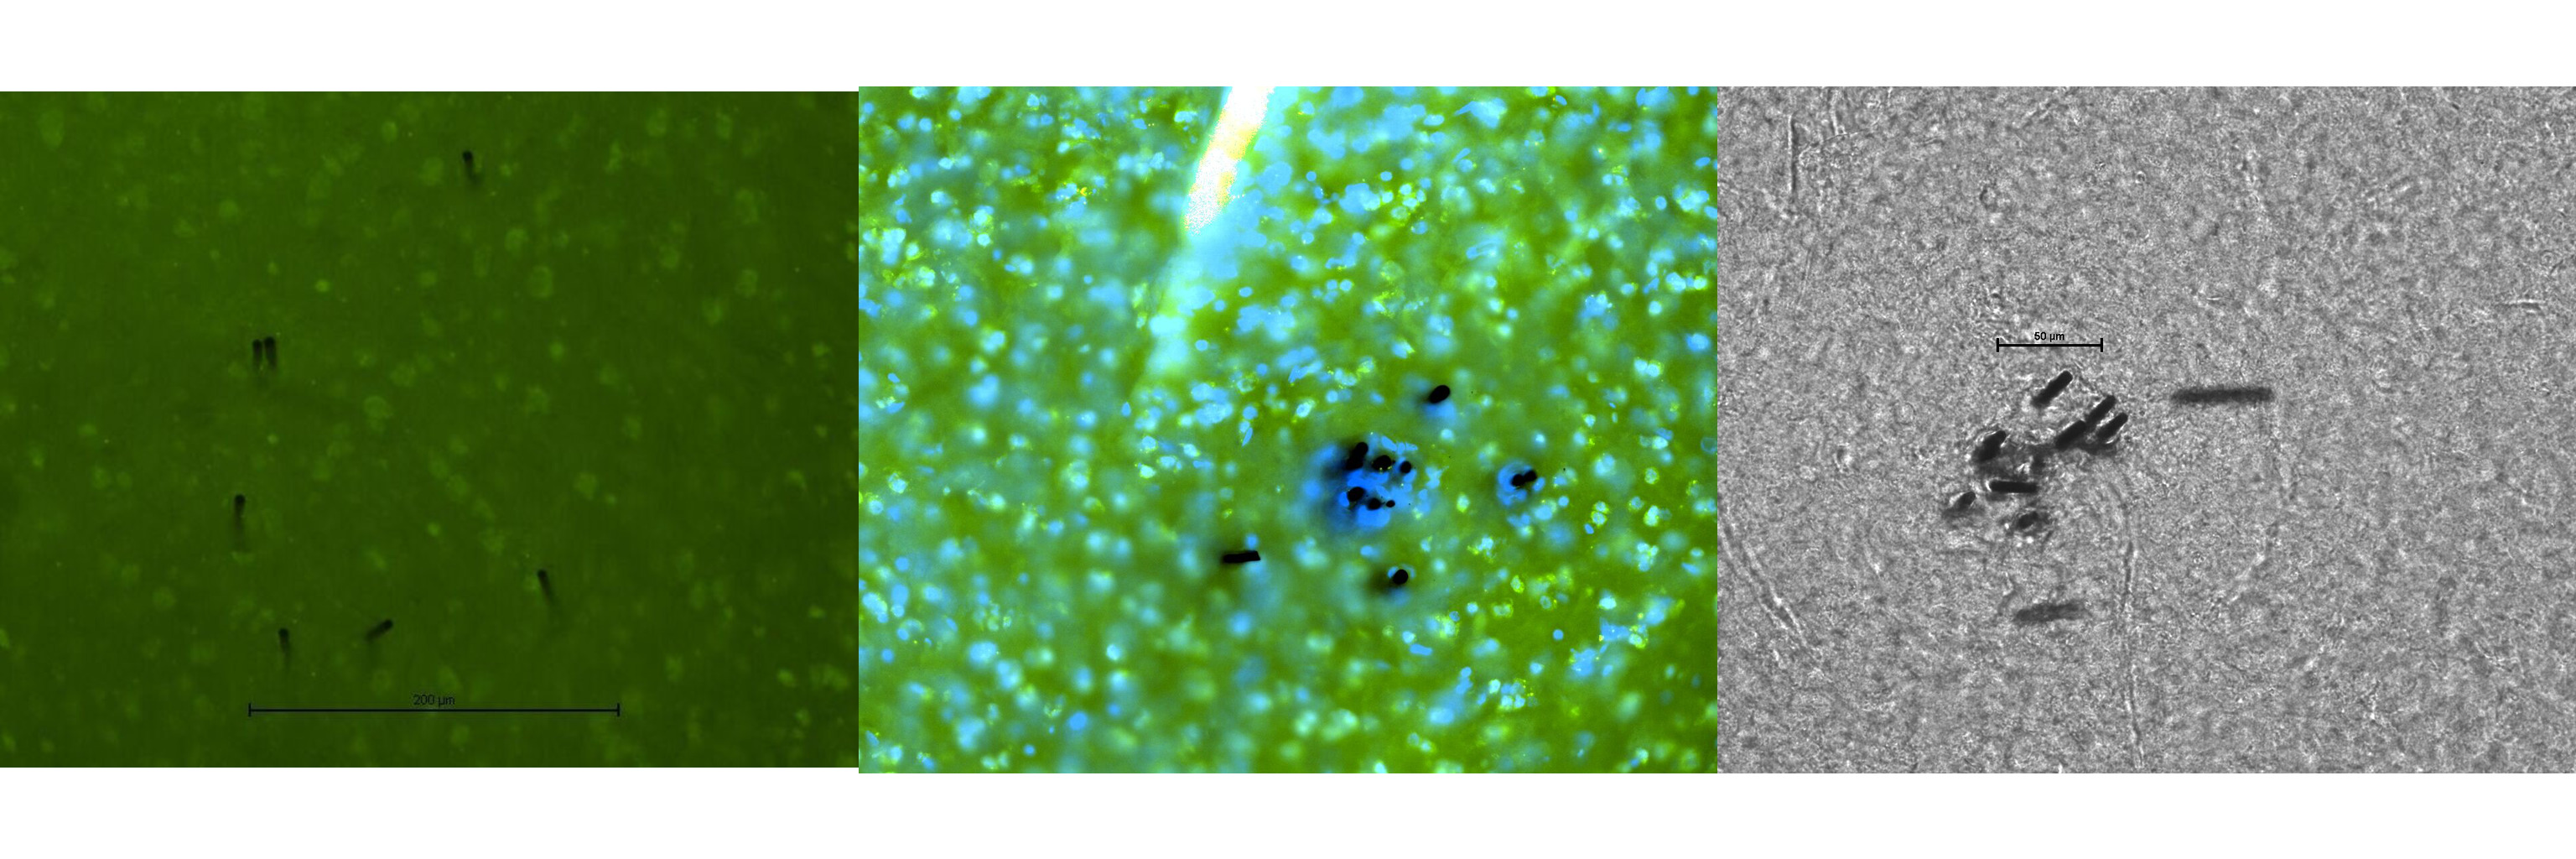
\includegraphics[width=\textwidth]{splay_montage}
  \caption{Splay types, left to right: examples of full splay, partial
    splay, and clumped.  In all images, black circles are electrode
    shafts; in many cases the slicing plane is not quite orthogonal to
    the electrodes, yielding oblong images.  In the bright-field image
    on the right, three of the electrode slices were pulled out of the
    tissue during slicing, and appear to lie flat on the slide.  Since
    their original locations cannot be determined, we have ignored
    them.}
  \label{fig:splay_montage}
\end{figure}

\marginpar{Would it make sense to automatically cluster the splay data?  Or to change the criteria?  I can think of some changes\dots}


\subsection{Recording}

For electrophysiology (recording and stimulation), birds were anesthetised with 1.5\% isoflurane, 98.5\% oxygen, at 0.5 liters/minute.

Recording of spontaneous activity in Area X was with an Intan RHD2000 amplifier at 20 kHz, with a high-pass filter at 200 Hz.  Recordings were broken down into data files 1 minute long.  Any data file with any sample whose absolute value was $>500$ $\mu$V was assumed to have excessive recording noise, and was discarded.

\subsection{Stimulation: Zebra finch antidromic HVC $\leftarrow$ X}

A common technique for
locating HVC in the zebra finch involves implanting a stimulating
electrode in Area X and looking for an antidromic response, which is
visible in HVC and not in the surrounding tissue
\cite{Swadlow1998antidromic,Hahnloser2002sparse}. We use this standard procedure as a starting point for an exploration of stimulation techniques.

For discussion of the stimulation paradigm, we will use the following definitions:

\begin{description}
\item[Channel:] Our electrodes have 16 channels, each of which is an individual carbon fibre connected to its own amplifier.
\item[Pulse:] A biphasic charge-balanced square wave of current.  Each phase is 200 $\mu s$ long, and there is no interpulse interval.
\item[Current steering:] Delivering pulses, possibly of opposite signs, to two or more electrodes simultaneously in order to control the geometry of current flow through the tissue.
\item[Current-steering configuration (CSC):] The configuration defining which channels receive the positive half of their biphasic pulse first, or vice versa.
\item[Pulse train:] A sequence of $n$ (usually 10) identical current-steered stimuli delivered to all active channels, usually at 25 Hz.  This is slow enough that pulses do not interfere with each other, and is used to measure the repeatability of the response.
\item[Threshold scan:] A series of pulse trains, each of which has the same CSC but a different current magnitude, designed to find the minimum current magnitude for this CSC that will induce an antidromic response in HVC.  The algorithm is described below.
\item[Voltage scan:] The Plexon hardware can deliver a current-controlled pulse to each of 16 channels independently and simultaneously, but only allows monitoring of the voltage delivered on one channel at a time. A voltage scan involves sending the same pulse train once per active electrode, monitoring a different one each time.
\end{description}

The stimulation and recording electrodes use separate electrical
returns, consisting of silver wire in contact with the
skull.  Some CSCs balance current delivery between the electrodes,
whereas others do not, and in the latter case excess current flows
through the common return.

We used a Plexon stimulator to control stimulation in Area X, and
recorded from HVC using a Tucker-Davis Technologies (TDT) RZ5
BioAmp processor with a Medusa preamplifier, or an Intan RZ2000\marginpar{Model \#? Also depending on
  which recording to show in \fig{fig:clear_hvc_response}}.  The
stimulator's self-monitoring channels were recorded on a National
Instruments (NI) PCI-6251 data acquisition card using the
session-based interface of Matlab (various versions from 2014a through
2015b) on Windows 8.1.

Electrical stimulation saturates the brain---including at the site of
the recording electrode, and thus also the recording amplifier---for some time post-stimulation. The time required for the amplifier to decay to baseline results in a stimulation artifact in the recording traces for 1--5 ms post-stimulus (with the TDT).
\marginpar{Intan} Responses to stimulation can be
detected outside of the saturation window and inside the decay region with appropriate de-trending. Since HVC and Area X are separated by about 5 mm, this response occurs 3--8 ms after
stimulation\cite{Fee2004mechanisms}\marginpar{Do you have a better citation?}, which usually gives the TDT amplifier time to settle before the response---at least sufficiently that the voltage traces may be effectively de-trended.


Custom MATLAB software controls the experiment, initiating spike train
delivery and response monitoring.  The Plexon's self-monitoring
channels are recorded by the NI card, and the neural response in HVC
is recorded by the TDT.  In order to guarantee precise temporal
alignment between stimulus delivery and response measurement, all
hardware is triggered by a TTL pulse from the NI card when it begins
its acquisition cycle.  The Plexon begins stimulating upon receipt of
that TTL pulse, and the TDT begins recording at 24.414 kHz (the
device's native frequency) on the same signal.  Whenever the Plexon is
actively delivering current (i.e. during each pulse within the train)
it sends out its own TTL pulse: this signal is recorded by the TDT
along with the HVC electrode voltages.  Thus the data alignment
precision is controlled by the sampling rate of the TDT (41 $\mu$s).

Programming each of the stimulator's 16 channels for one pulse train and running the train (10 pulses at 25 Hz) requires a little under 4 seconds. A threshold scan requires, on average, around 15 pulse trains, and so generally takes around a minute. Likewise, a voltage scan requires delivering one pulse train per active electrode, for a total of another minute.\marginpar{This timing is before I did some speedup hacking---it's nearly twice as fast now---but most of the data shown here were gathered pre-speedup. Does it matter?}

\subsubsection{Response detection}
\label{sec:responsedetection}

HVC projects into Area X (and into RA, which we do not discuss here).
When Area X is stimulated, an antidromic response may be observed both
in HVC\textsubscript{X} projection neurons and in HVC interneurons.
The antidromic response occurs roughly 3--8 ms after the stimulation
pulse, and is highly stereotyped: \cite{Fee2004mechanisms} reports
that the variability in the timing of the antidromic response in
HVC\textsubscript{X} projection neurons is under 50 $\mu$s, while that
of HVC intraneurons is above 500 $\mu$s.

\fig{fig:clear_hvc_response} shows an example of a pronounced HVC
response to stimulation in Area X.  We detected such responses in two different ways, one during experiment runtime and one in postprocessing analysis:

During runtime (threshold and voltage scans), we measured the
cross-correlation between the recorded response for each pulse in a
train and each other with a maximum lag of 100 $\mu$s (note that our recording amplifier samples every 41 $\mu$s), which provides
a robust way of separating the response of projection neurons from
noise.  Because the HVC amplifier's (Intan's or TDT's) response to the
transient stimulation pulse in Area X can persist into the time of
interest (3--8 ms), each response is first de-trended using a
maximum-likelihood fit over the region 2.5--25 ms using an eigth order
Fourier series, which removes post-stimulation decay while leaving
spike-sized signals intact.\marginpar{Filtering would probably work
  better with the TDT than with the Intan\dots} We found that this
strongly biased smoothing technique more cleanly removes the large
stimulation artifact than the conventional approach of
bandpass-filtering the signal. The cross-correlation threshold above
which a response is identified is chosen by visual inspection.

A further, independent voltage-threshold analysys was performed offline.  For each train of $n$ pulses, we labeled peaks greater
than 5 standard deviations from the RMS noise of a nearby (within 20
ms) non-stimulated recording on the same electrode.  For each of the
$n$ stimuli in the pulse train, all peaks' delays post-stimulus were
compared to those from the other $n-1$ responses, and any peak whose
delay was within 100 $\mu$s of another peak was considered a response
to the stimulus.  The probability of a response at this current was
then the maximum number of aligned peaks divided by the number $n$ of
pulses in the train.  Given the set of points
Pr(response$\,\,|\,\,$maximum electrode voltage), we then fit a
sigmoid $0.5 (1 + \tanh(\lambda(x-\mu)))$ to this curve, and take the
midpoint $\mu$ as the voltage required to induce a response with
probability 50\%.

\begin{figure}
  \includegraphics[width=\textwidth]{lw95rhp-2015-08-05_18.39.07.eps}
  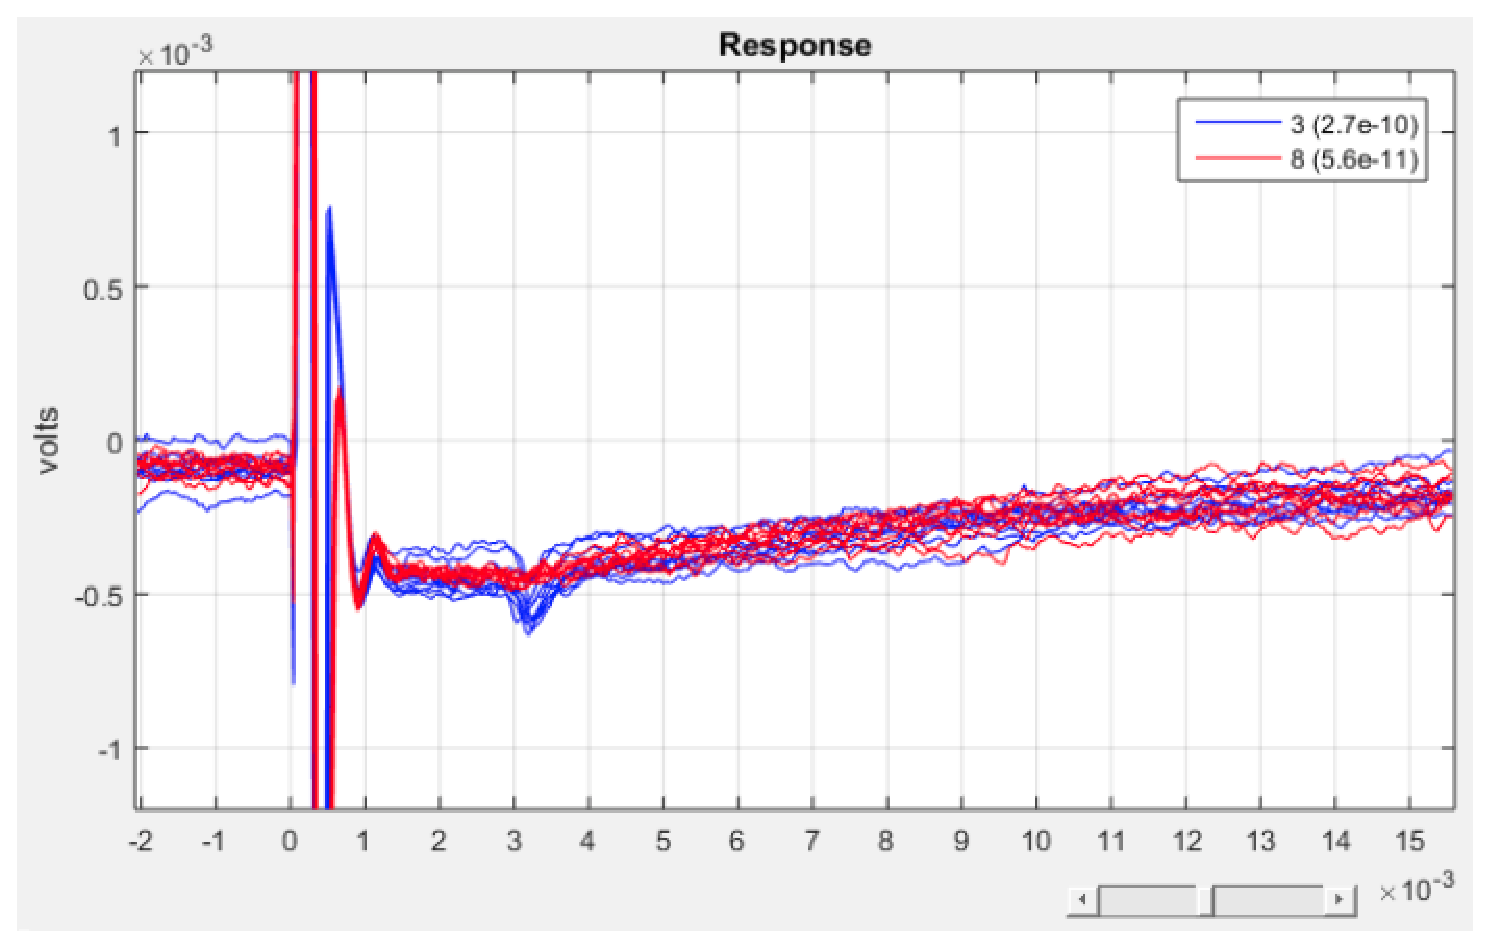
\includegraphics[width=\textwidth]{lw95rhp-2015-12-02}
  \caption{An example of a strong response in HVC.  {\bf Top:} The
    horizontal axis is time in milliseconds relative to the onset of a
    stimulation pulse.  Here, the stimulation is a 400-$\mu$s biphasic
    pulse of 3 $\mu$A, in which voltage peaked at 1.6 V.  Stimulation
    was repeated 20 times at 25 Hz, with each response aligned to its
    respective pulse to within 41 $\mu$s.  Various response activity
    can be seen, but the most pronounced is at 6.2 ms post-onset.
    {\bf Bottom:} a different bird, with a much weaker signal, but
    recorded on the TDT.  200 $\mu$s, 6.94 $\mu$A, 1.2 V peak.{\em Use the
      top figure?  It only shows one channel, and it's recorded on the
      Intan, which I was using while the HVC signals were still
      pretty.  That means a lot worse amplifier settling, so it's not
      the best image, but the response is much cleaner than later ones
      made with the TDT.}}
  \label{fig:clear_hvc_response}
\end{figure}

As the bird ages, the implant bonding site is slowly pushed away
from\marginpar{Details or citation?  Possibly
  \cite{Barrese2016electrodestability}, although they don't really
  discuss this so much.} the skull.  For shallow installations such as
HVC (depth $\approx 200$ $\mu$m, the quality of the HVC recordings
diminishes as electrodes are forced out of contact with the brain.
This makes it more and more difficult over time to measure the
antidromic response.  The above cross-correlation technique for
response detection is more sensitive than the method typically used
during acute or short-term response measurements, in which a
pronounced spike is often clearly visible and is identified by eye on
an oscilloscope.  We are confident that we are measuring an antidromic
response because it is on the correct timescale both in delay
post-stimulus and in consistency, appears near the expected
stimulation threshold, and has the expected shape.\marginpar{Cite
  papers giving timing and stimulation threshold.}

\subsubsection{Threshold scan}

What stimulation parameters are required in order to reliably elicit
an antidromic response to stimulation in Area X?  How can this
threshold be found quickly, while minimising the risk of exceeding
safe stimulation voltages?  How can this process be made robust to
noise?\marginpar{How can we establish how much robustness to noise is
  required?}


After choosing a CSC, we begin stimulating at a current that is known
to be below threshold.  While no response is seen, the current is
increased gradually by a small factor $\alpha = 1.1$ until either a
response is detected or the voltage or current limit is exceeded.  In
the latter case, a lack of response is reported, and we move on to the
next CSC.  If a response is found, then the step size is decreased
towards unity ($\alpha \leftarrow \alpha^{2/3}$) and we reduce the
current until the response disappears.  This process is repeated until
the step size drops below a limit ($\alpha < 1.02$), and the threshold
is taken as the last parameter set that induced a response.

While a larger step size would result in a faster search, and a binary
search would additionally be easier to describe, this ad-hoc approach
samples near the current of interest while making it unlikely that we
will stimulate with a current that significantly exceeds the minimum
required for a response, and thus minimises the possibility of
injuring the bird.

\subsubsection{Voltage scan}

Once the minimum current required in order to achieve a response is
identified, we perform a voltage scan at that current, in order to
measure the peak voltage delivered to each electrode. Since the ratio
of voltages over the electrodes tends to remain fairly constant, the
electrode that reached the highest absolute voltage in the previous
scan is used for the overvoltage termination condition.

\section{Results}

\subsection{Splay histology}

After exclusion, 22 arrays, implanted into 13 different birds, each
yielded at least 3 measurable electrodes.  See
Table~\ref{table:splaydata} for the raw data and \fig{fig:splaydata}
for visualisations thereof.\marginpar{Perhaps take out the table and
  just use the graphs?}



\begin{table}
  \begin{tabular}{cccc}
    & \multicolumn{3}{c}{Inter-electrode distance ($\mu$m)} \\
    \# Good electrodes & Mean & StdDev & Max \\
    \hline
     3  &  5.0    &    0 &  20.0 \\
   10  &  6.0   & 2.1 &  52.9 \\
   16  &  6.3   & 6.3 &  48.3 \\
    4  &  7.5   & 5.0 &  35.8 \\
    6  & 16.7  & 18.9 &  44.8 \\
    9  &  7.7   & 5.5 & 107 \\
   14 &  12.8  & 12.1 & 15.2 \\
    8 &  14.7  & 17.8 & 108 \\
   15&   15.1  & 10.2 & 163 \\
   15  & 19.3  & 19.1 & 128 \\
    5  & 22.0  & 27.7 & 103 \\
    9  & 28.2   & 35.8 & 148 \\
   11 &  31.8  & 28.1 & 103 \\
    8  & 35.9  & 30.6 & 228 \\
   13 &  76.5 & 152 & 167 \\
    5  & 51.4  & 28.1 &  51.5 \\
    3  & 20.0    &     0 & 123 \\
    6  & 73.5  & 35.5 & 128 \\
    8  & 38.5  & 35.2 & 142 \\
    9  & 47.4  & 31.5 & 208 \\
    5 & 126  & 63.5&  214 \\
    16 &  62.0 &  58.9&  829
  \end{tabular}
  \caption{Raw data.  Each row shows the statistics from one electrode
    array.  ``Good'' electrodes is the the number of carbon fibre
    electrodes in each bundle that appeared to still be firmly fixed
    in the neural tissue after slicing.}
  \label{table:splaydata}
\end{table}

\begin{figure}
  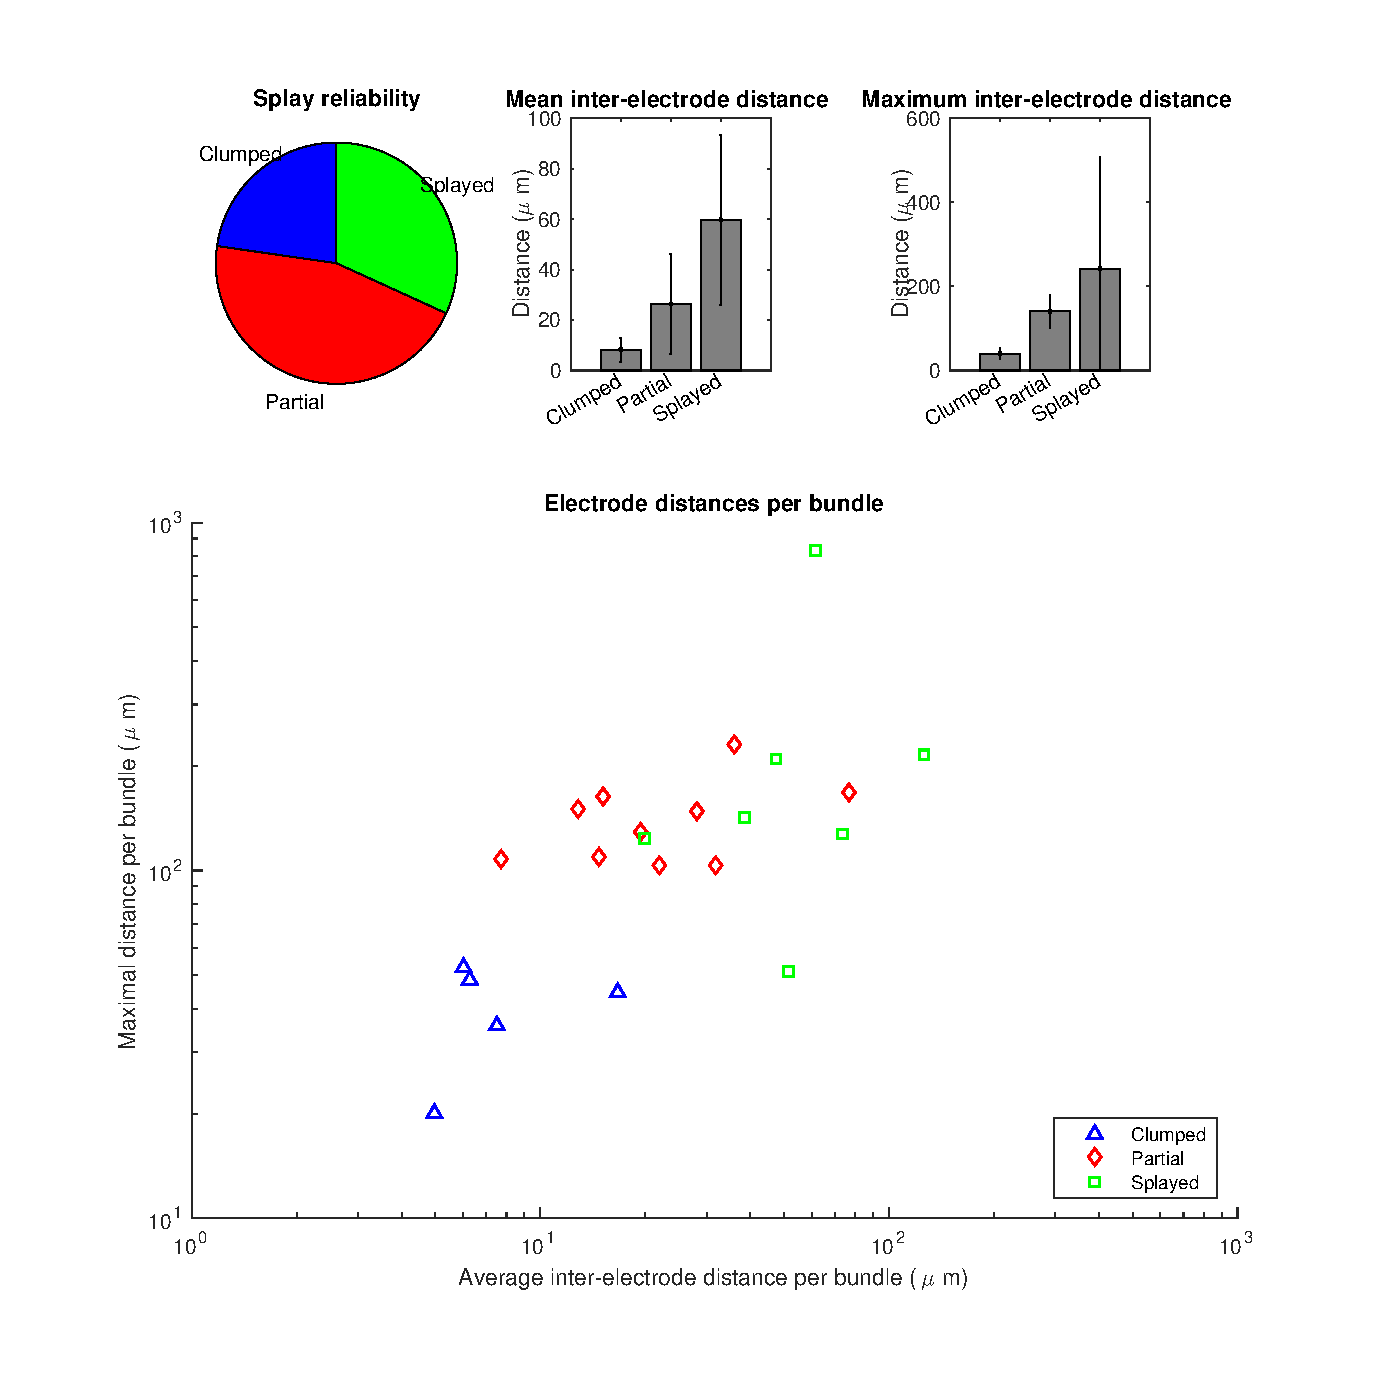
\includegraphics[width=\textwidth]{splay_data}
  \caption{Splay histology data from Table~\ref{table:splaydata}.}
  \label{fig:splaydata}
\end{figure}

\fig{fig:damage} shows some examples of the damage done to the brain
in the vicinity of the electrodes.\marginpar{An image of ``typical''
  damage done by ``micro''electrodes would be nice, but it's hard to
  show what's typical of the \sout{competition} prior work with any
  credibility.  Letting people compare vs.~their own experiences is
  the best, but not everyone (e.g. me) will know what's typical.}
\marginpar{I have data on how long post-implant the birds lived before
  these data were taken, which needs to come along with this figure or
  somewhere.}  Visual inspection shows little damage in the vicinity
of single electrodes, and slightly more in clumped electrode groups.
Visual inspection can give some indication of the damage done to the
brain and the likelihood of achieving good electrical contact with
neurons, but we are more interested in the ability to interact with
the brain (see Section~\ref{sec:results:recording}).

\begin{figure}
  % montage -geometry 1024x1024 DAPI-and-NeuN*.jpeg damage.eps
  \includegraphics[width=\textwidth]{damage}
  \caption{Typical damage.  Neural nuclei are shown in green (stained with
    NeuN) and all cells in blue (DAPI).  The presence of non-neural
    cells indicates damage, and is notable in the vicinity of the
    largest non-splayed electrode bundle, and nearly absent around
    individual electrodes.}
  \label{fig:damage}
\end{figure}




\subsection{Chronic recording}
\label{sec:results:recording}

\subsubsection{Impedances}

\marginpar{I think I have impedance data for Greg's latest electrodes, as well as pre-implant data for the ones shown in the following figures. This paper is not really about biochemistry, but that could all be thrown in\dots}

\fig{fig:impedances}
\fig{fig:impedances-all}
\fig{fig:impedances-lw95rhp}

\begin{figure}
  % Width 9, height 5, fonts auto (100%), lw94rhp
  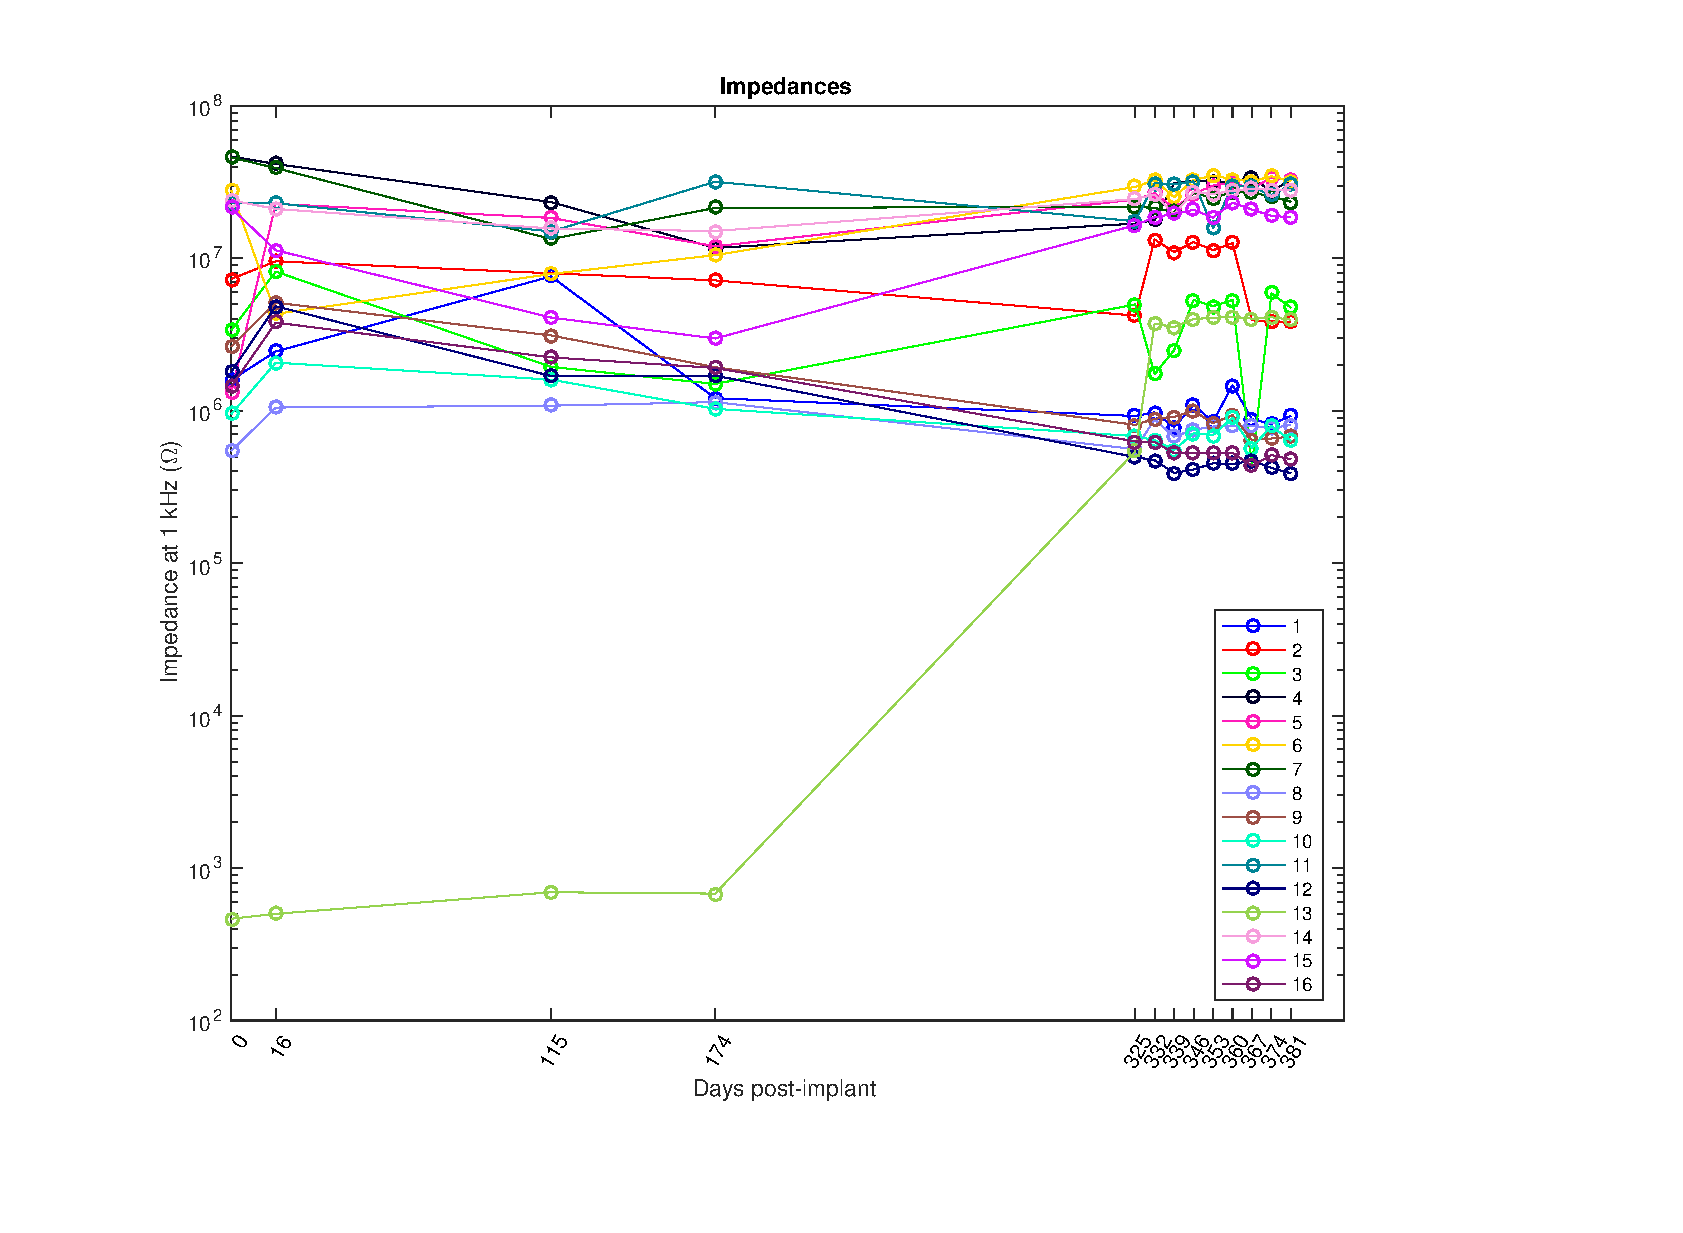
\includegraphics[width=\textwidth]{Impedances}
  \caption{Impedances for the electrodes shown in
    \fig{fig:XSpikeRecording}.  Most good electrodes were in the range
    400 k$\Omega$--1M$\Omega$ for the recordings shown in that
    figure.}
  \label{fig:impedances}
\end{figure}


\begin{figure}
  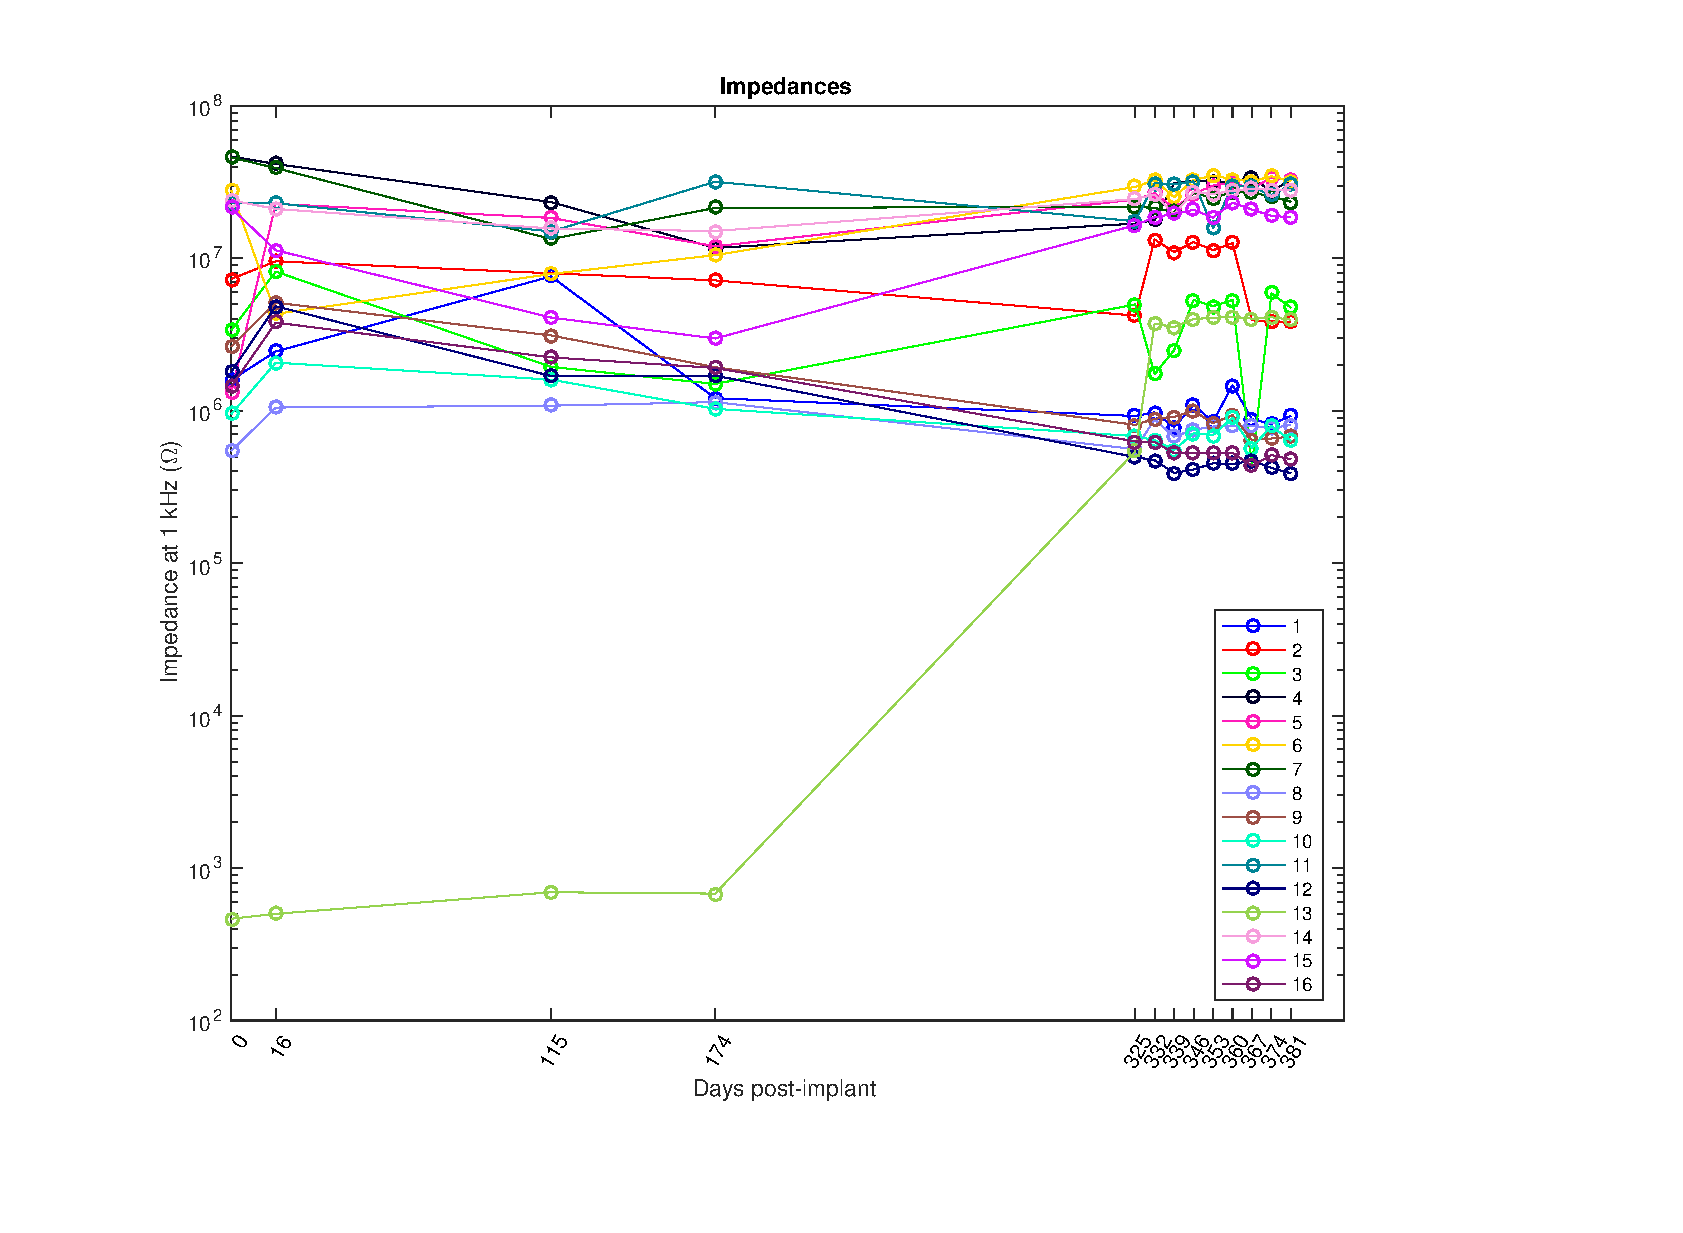
\includegraphics[width=\textwidth]{Impedances-all}
  \caption{{\em Full version of \fig{fig:impedances}.  I think I like this one less, but it could be more useful despite (or because of) showing a bunch of bad electrodes\dots}}
  \label{fig:impedances-all}
\end{figure}


\begin{figure}
  % Width 9, height 5, fonts auto (100%), lw95rhp
  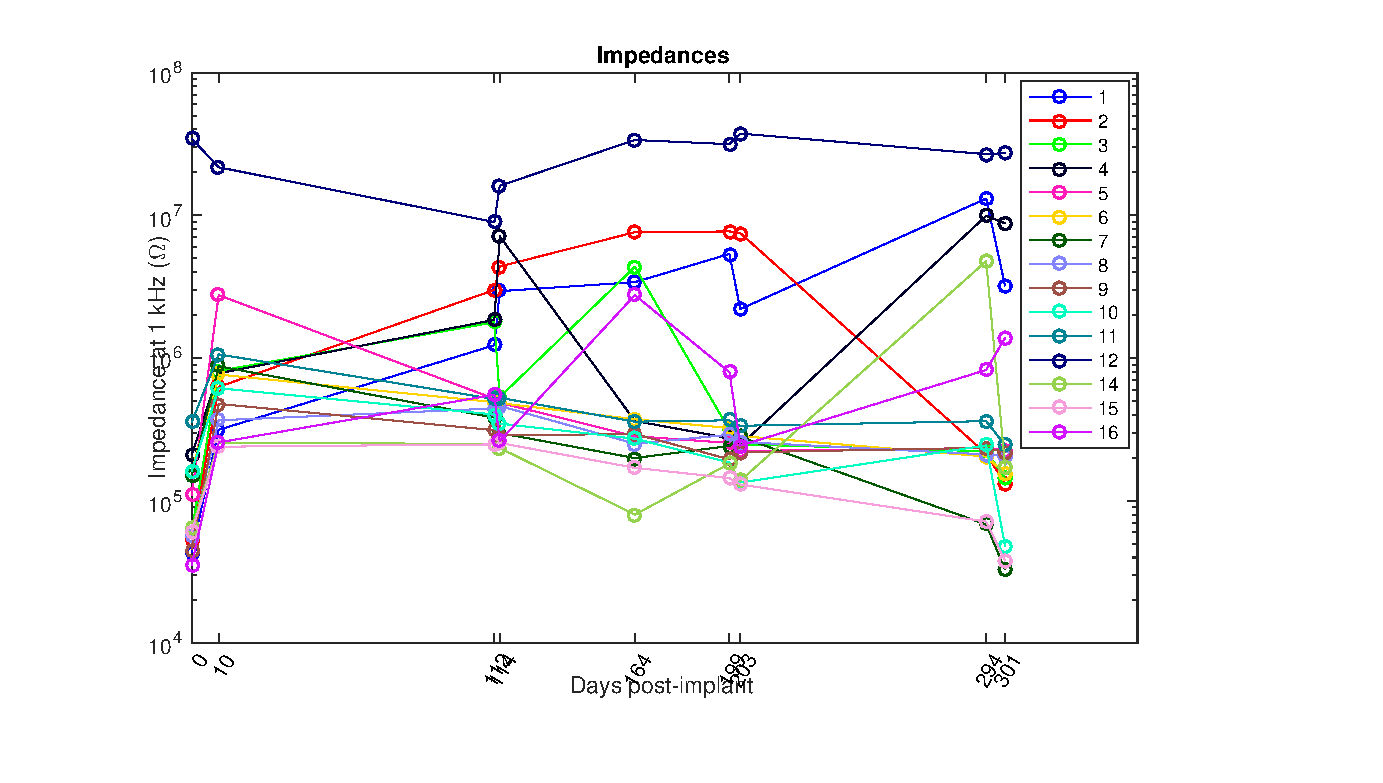
\includegraphics[width=\textwidth]{Impedances-lw95rhp}
  \caption{Electrode impedances over time on another bird.  This Area X array was treated with iridium oxide.  {\em This plot probably requires a bunch more explanation.  Notably: why the big jumps?  Need to check on stimulation, but hard to generalise with so little data\dots}}
  \label{fig:impedances-lw95rhp}
\end{figure}

\subsubsection{HVC}

Long-term recording in HVC is difficult due to skull regrowth
interfering with electrodes implanted only a few hundred microns from
the surface: after 10 months, we had difficulty picking up antidromic
response in our two remaining birds, as discussed in \sref{sec:responsedetection}. \marginpar{Duplicate. Omit?} 
  
\subsubsection{Area X}

More telling of the potential of these electrodes to detect spikes chronically is
the recording of spontaneous activity in Area X, which was still
easily seen in several channels after a year.\marginpar{I don't have
  recording-only data from early on. Oh---now I do! But in another
  bird. What about it to present?}  \fig{fig:XSpikeRecording} shows recordings a year after
implantation for the most stable electrodes of the 16.



\begin{figure}
  % Width 9, Height 9, Font scaling 100%, lw94rhp I think?
  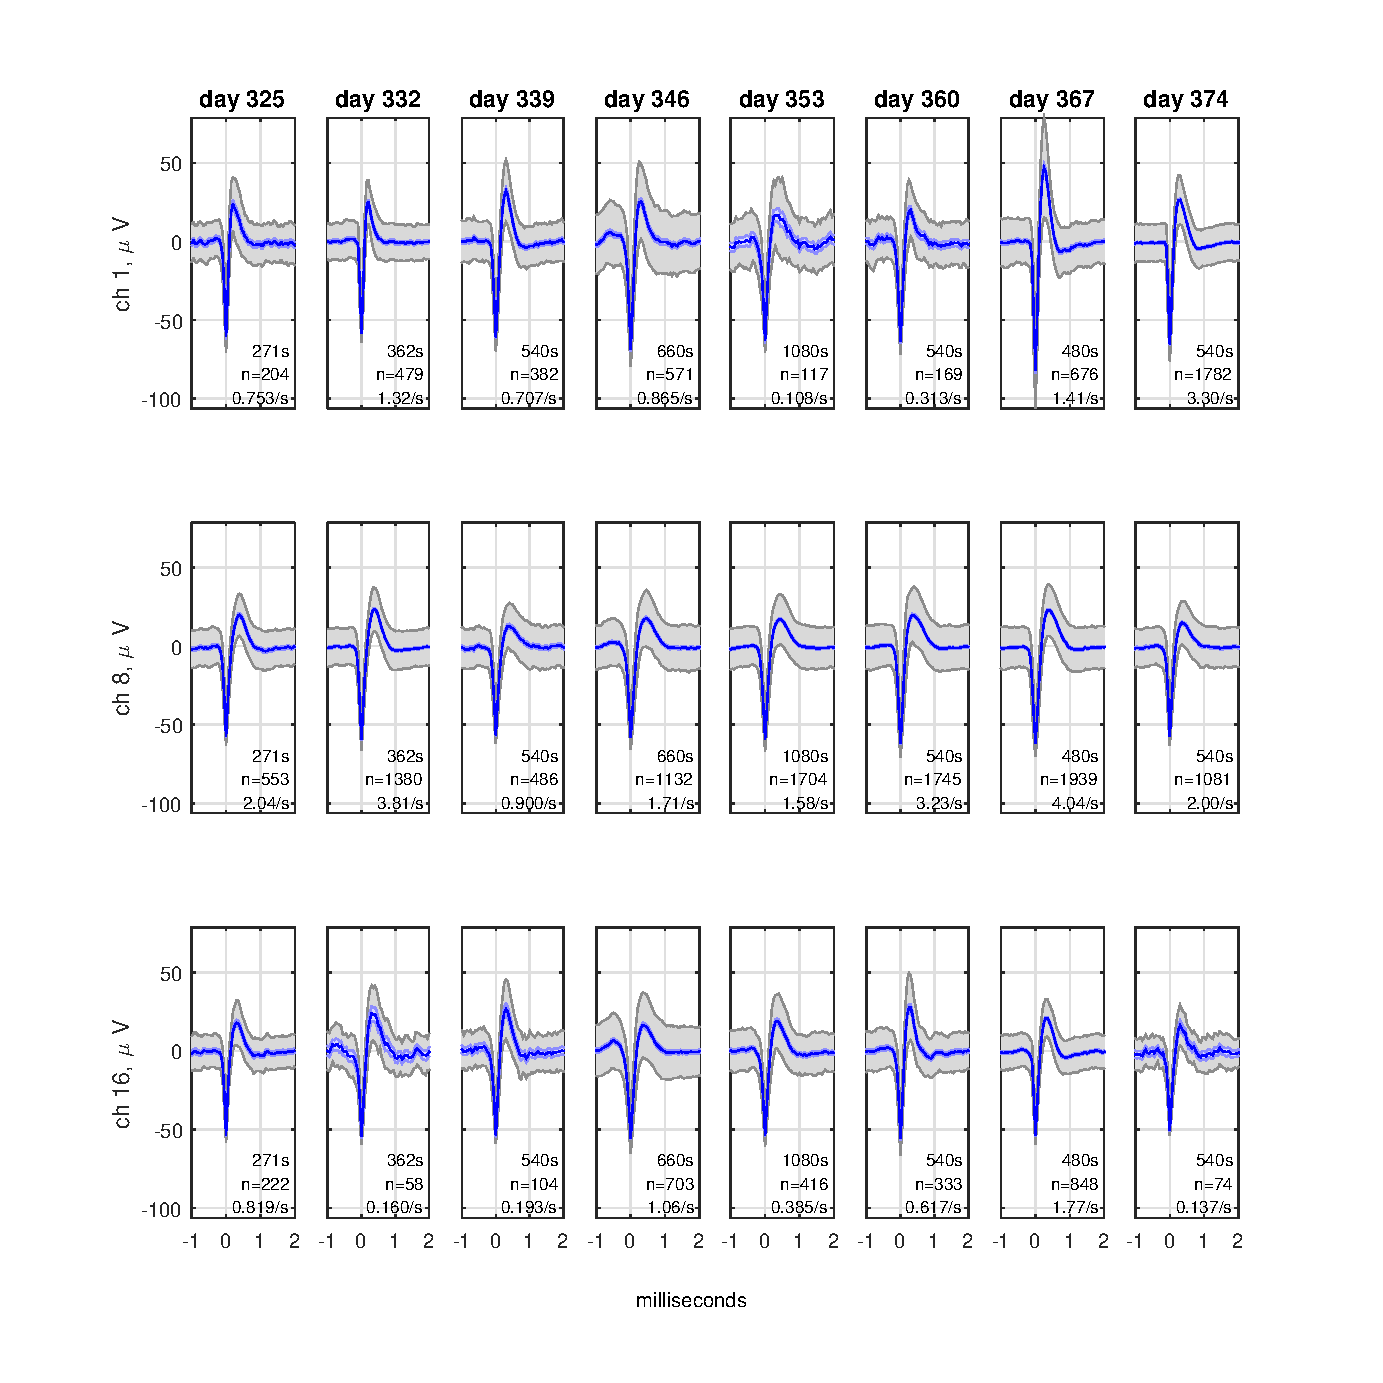
\includegraphics[width=\textwidth]{XSpikeRecording}
  \caption{{\em FIXME Here I show 6 electrodes.  3 are beautiful, and
      3 fade in and out.  What's the best way to present this?  Should
      I omit graphs with fewer than 20 spikes as I've done here Or
      show their messy squiggles?}  Some of the electrodes in Area X
    record spontaneous spikes a year after implantation.  Column
    titles show the number of days since implantation and the number of seconds of
    recorded data.  Each row is one electrode (shown here: the three
    most stable channels and three that showed some variability).
    Legends show the number of seconds of the recording, the number of
    spikes, and mean spike rate.  The grey shaded region is standard
    deviation, and the coloured shaded region is the 95\% confidence
    interval for the mean. {\em FIXME Are these the same spike?}}
  \label{fig:XSpikeRecording}
\end{figure}




\subsection{Stimulation}

\subsubsection{Minimising stimulation voltage}

Some CSCs required lower currents to induce the antidromic response
than others. In lw94rhp, 11 electrodes were undamaged. From the
$2^{11}$ possible CSCs we chose 32 (30 randomly, and the two that
treated all electrodes identically).  For each CSC, we performed a
threshold scan to find the minimum current needed to trigger a
response.  When this current was found, we did a voltage scan.  We
tested the sequence of all 32 CSCs five times on an anesthetised bird.  Results are shown
in \fig{fig:VoltageVsCSC}.  The best CSCs resulted in a maximum
voltage of around 1~V, while the worst were over 2.5~V.  Perhaps
surprisingly, the CSCs that sent identical pulses to all 11 electrodes
were among the worst performers, with our simple search revealing CSCs
that kept voltages far lower.

The maximum-likelihood fits to the voltage sweep data (green errorbars
in \fig{fig:VoltageVsCSC}) consistently yield slighly higher threshold
voltages than those measured using the search.  This is because
whereas the maximum-likelihood fit computes the voltage required in
order to obtain a response with 50\% probability, the threshold
search, which guided data acquisition in realtime, looks for any
significant correlation between the responses in each spike train,
which is detectable well before the stimulation achieves a 50\%
response rate.

\noprint{FIXME: The following caveat doesn't apply to
  lw95rhp-2015-12-04: Each threshold scan terminated when a
  stimulation voltage over 3 V was detected, so for some datasets
  (e.g. lw95rhp-2015-12-09) we were unable to acquire all five
  measurements for some CSCs, and thus they are worse than the figure
  shows.}

\begin{figure}
  % plot_max_voltage_bar.m, reanalyse_thresholds.m
  % lw95rhp-2015-12-04 (data also available on -09 and lw85ry-2015-12-17)
  % width 7 in, height 6 in, fonts auto
  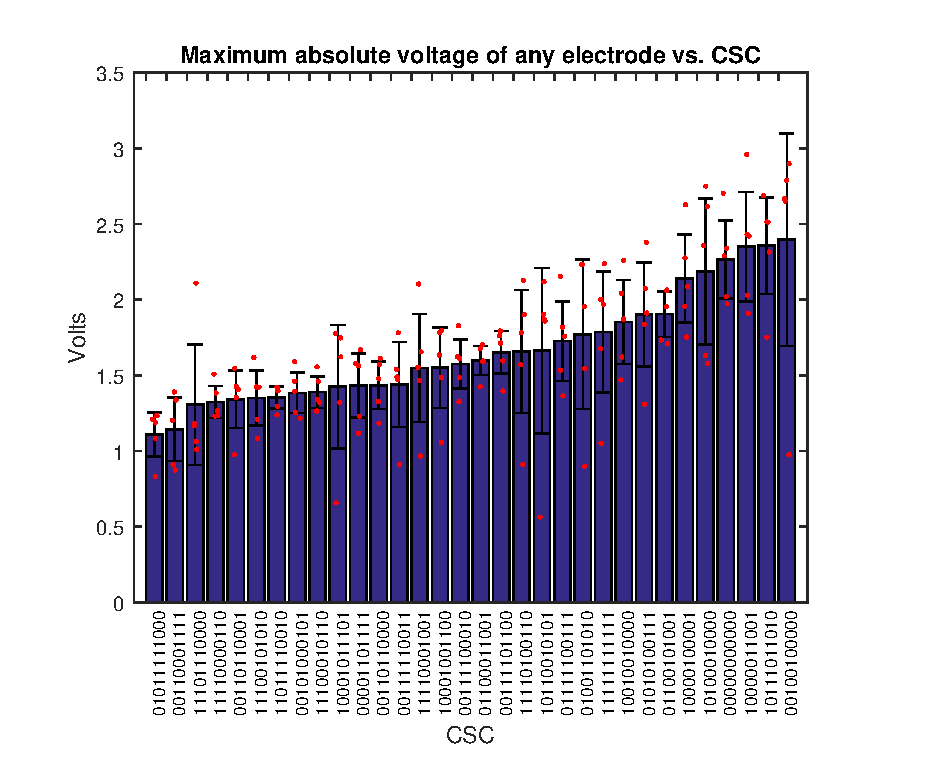
\includegraphics[width=\textwidth]{VoltageVsCSC}
  \caption{The peak Area X stimulation voltage required in order to
    achieve biologically effective levels of stimulation in HVC varies
    with different current-steering configurations.  Here are 32
    different configurations, over 5 trials each, taken 214 days
    post-surgery.  The X axis lists the configuration (each of the 11
    active electrodes delivers a positive-first ``0'' or
    negative-first ``1'' current-controlled pulse).  The Y axis shows
    the maximum voltage across any electrode for the given CSC at the
    lowest current that evoked a reliable response.  Blue bars are the
    mean voltage discovered using the online threshold scan technique
    described in Methods, red dots show the voltage result for each
    trial, and error bars are 95\% confidence intervals (n=5).  Green
    bars show the voltage required to induce 50\% probability of
    response using a the maximum-likelihood analysis described in
    Methods, also as 95\% confidence intervals (when the confidence
    lines would have spanned the whole range of the graph, they have
    been omitted for clarity), and with crossbar marker at the mean,
    with marker width chosen to give an approximate sense of
    confidence. {\em FIXME Cosmetic stuff: xlabel/ylabel collisions, expand Y axis, maybe angle the CSCs, and why a bar graph?}}
  \label{fig:VoltageVsCSC}
\end{figure}

\subsubsection{Controlling the antidromic response}

Different CSCs delivered to Area X resulted in different response
patterns in upstream area HVC, as can be seen by the representative
examples in \fig{fig:HVCresponseVsCSC}. Besides providing further
evidence that the electrode arrays splayed, this suggests that the
approach might be able to induce specifically designed neural dynamics
beyond simply the presence or absence of a response.

\begin{figure}
  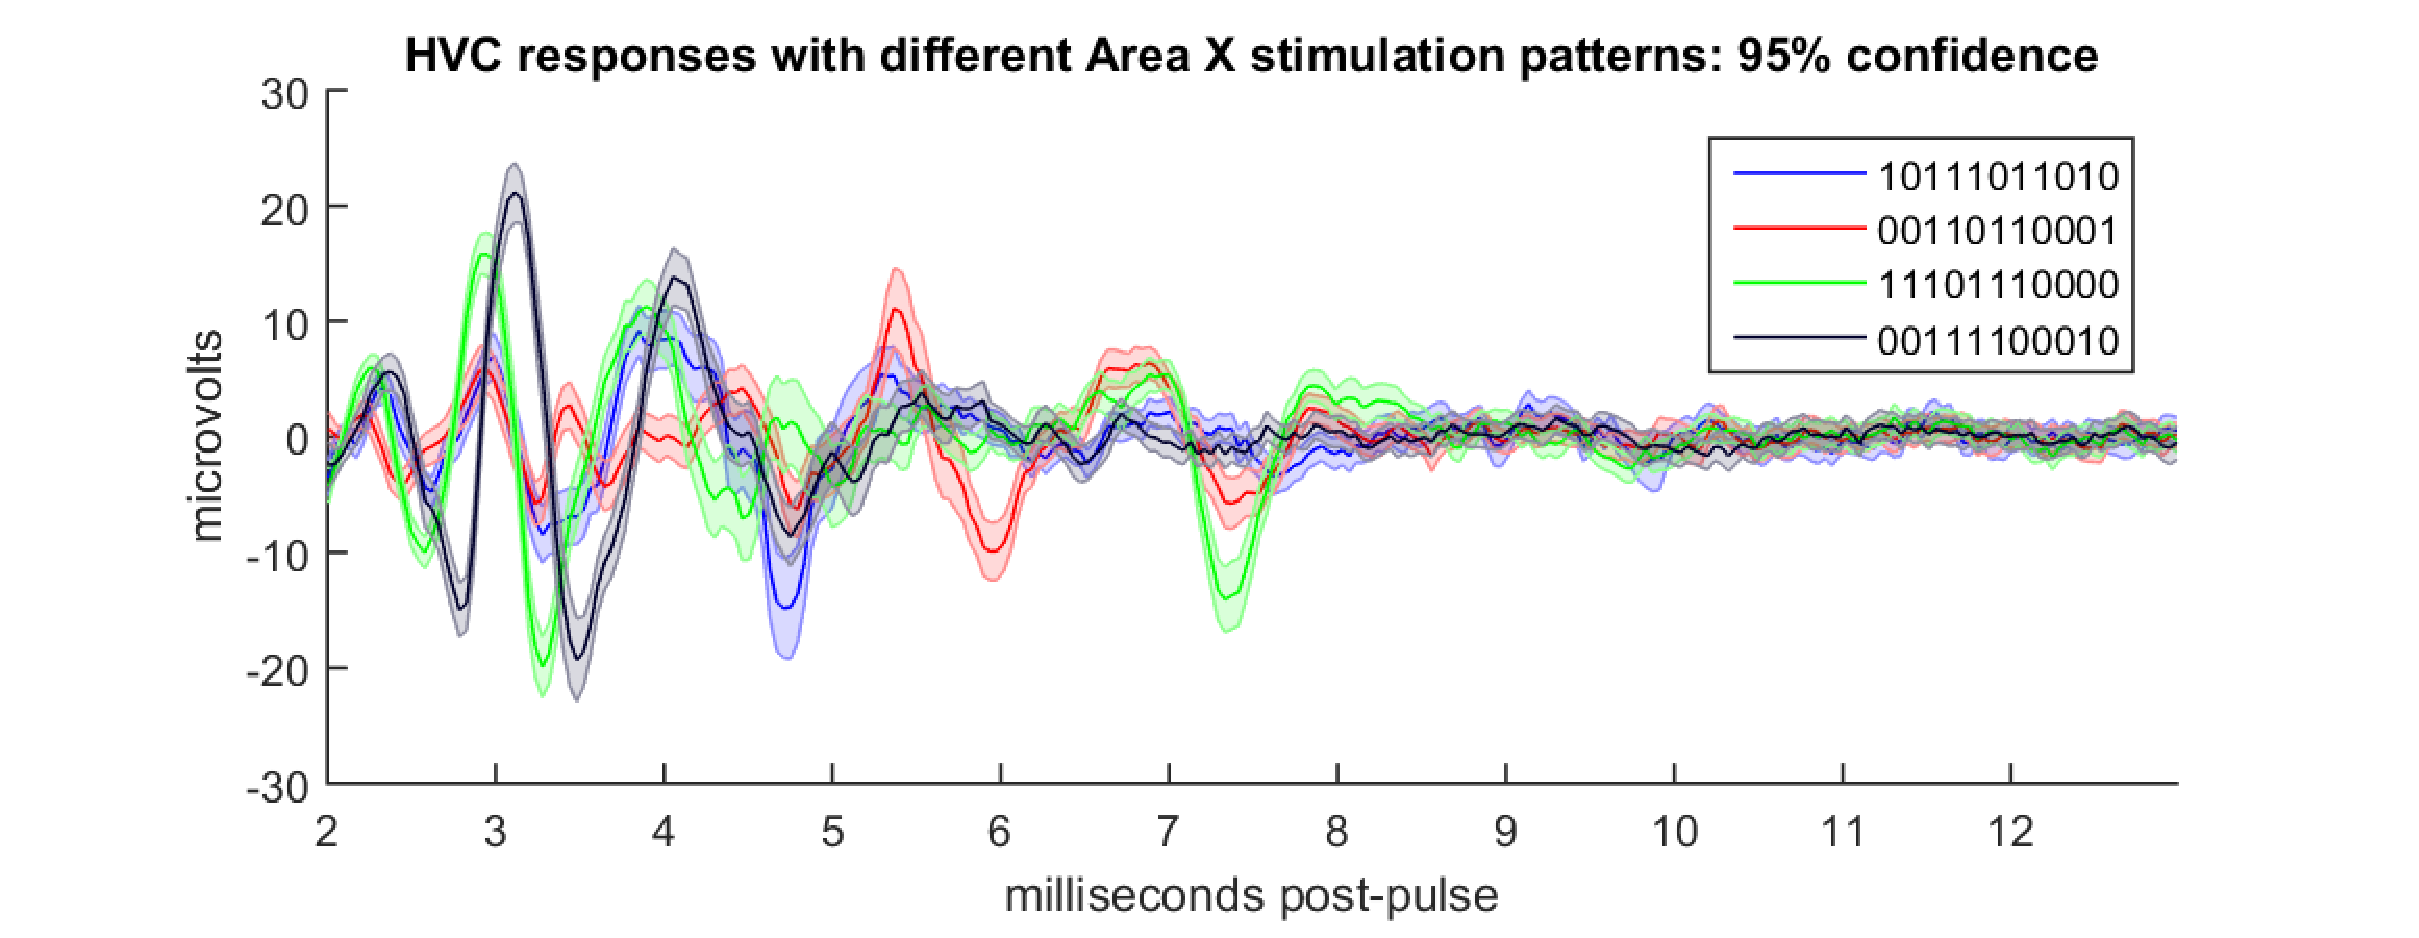
\includegraphics[width=\textwidth]{HVCresponseVsCSC}
  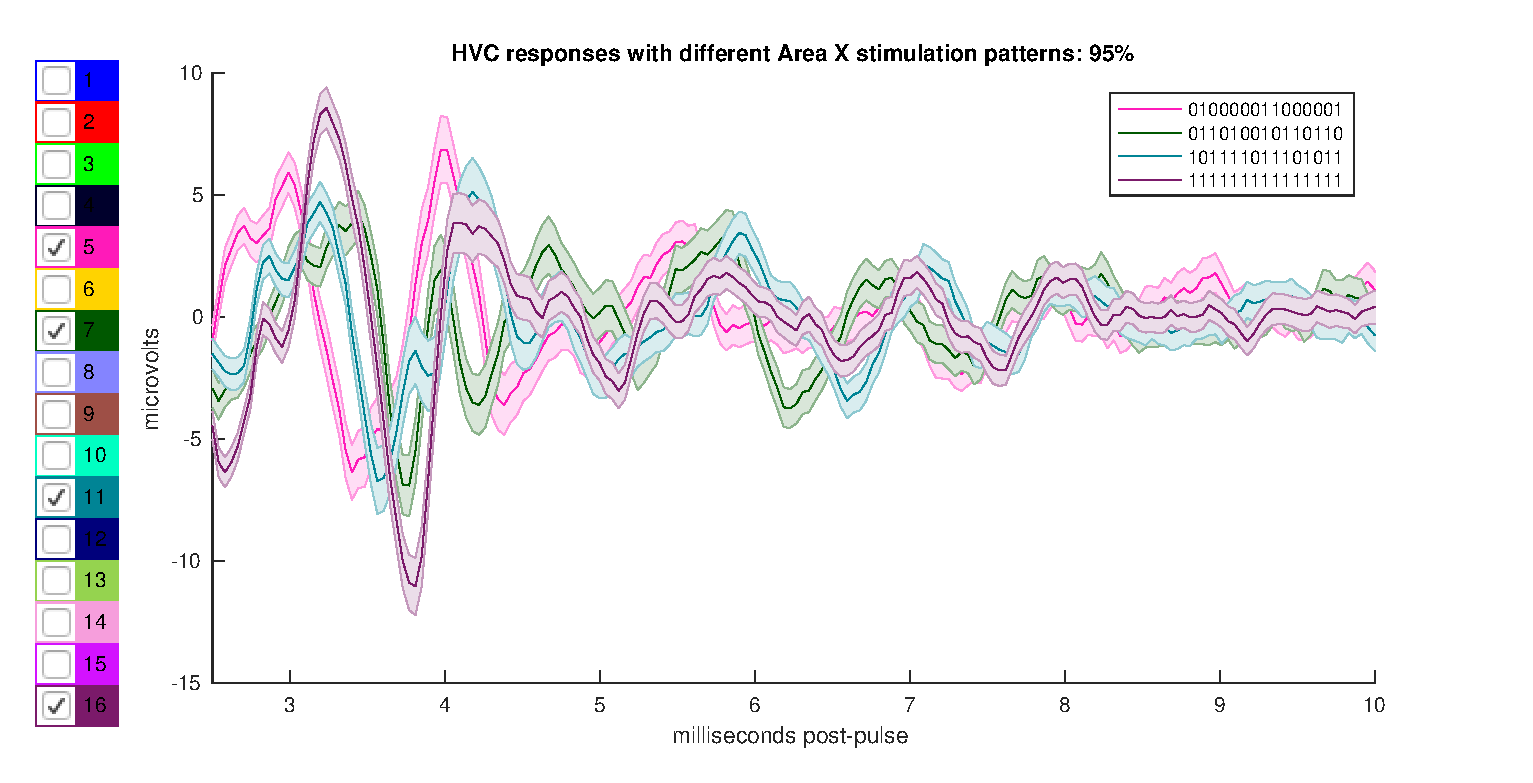
\includegraphics[width=\textwidth]{lr7-unique-responses-10-07-a}
  \caption{Different CSCs delivered to Area X can induce different
    responses antidromically in HVC.  {\em Top:} four of the most
    distinct responses to four of the 32 CSCs shown in
    \fig{fig:VoltageVsCSC}, bird lr95rhp {\em FIXME Right bird?}.
        {\em Bottom:} four distinct responses in bird lr7. Shading is
        95\% confidence, n=198 {\em FIXME n for lr7?}.}
  \label{fig:HVCresponseVsCSC}
\end{figure}


\section{Discussion}

\subsection{Splay}

Achieving consistent splay with these electrode arrays has proven difficult---the spatial distribution of electrodes is highly variable. Nonetheless, they splay well enough often enough to suggest that the design should be investigated further, especially given the state-of-the-art minimal damage and encapsulation.

\subsection{Steering}

\cite{Jepson2014steering_in_retina} showed good capacity to control
stimulation by steering current between electrodes in monkey retina,
allowing targeting of neurons on a smaller scale than the electrode
spacing.  The demonstration of fine control is compelling, but whether
or not the locally linear predictive response model that they found
effective in retina would be extensible to regions with greater
lateral connectivity is unknown.

Injecting current into tissue causes neurons whose axons are very
close to the stimulation site to fire, rather than neurons whose
bodies are at greater distances \cite{Histed2009stimulation}.  As a
result, the set of neurons that respond to a stimulation pulse is
highly sensitive to electrode location, but has spatial extent similar
to that of the neuron's dendritic tree.  Furthermore, they showed that
neurons stimulated in this manner seldom stimulate downstream neurons
synaptically.

Splaying electrode arrays with learning stimulation software may be
able to exploit these properties.  First consider each of the $n$
electrodes in our array separately.  $n$ sites stimulated at a given
current yields up to $n$ different random sets of $k_n$ neurons that
will fire, and increasing the current changes the size of $k$.  There
may exist multiple downstream neurons $y$ such that
directly-stimulatable neurons from several of our $n$ sets synapse
onto $y$.  This creates a search problem: how to stimulate the $n$
sets in a way that reliably stimulates $y$ enough to cause it to
spike, while minimising unwanted activity? This requires search over
current delivered to each group in $n$ in order to control which
neurons are recruited, and timing of stimulation delivery to each
group in $n$, so that appropriate downstream neurons are reliably
triggered.  Different values of current and timing delivered into the
$n$ groups may trigger different downstream neurons, so one possible
search problem is finding as many different downstream neurons as
possible.

Furthermore, it seems likely that directly-stimulatable neurons may
synapse onto others that are directly-stimulatable, once or $r$ times
removed. This suggests a more general objective for the search, in
which different timings for stimulating the $n$ sets may trigger
different network-scale dynamics (the same mechanism in the context of
current steering in retina\cite{Jepson2014steering_in_retina} is
related).  This greatly enlarges the space of inducible dynamics, and
also suggests the possibility of inducing Hebbian learning, which we
presume would tend to magnify and stabilise the effect of such
stimulation over time.\marginpar{Wild speculation. Too much so?}

Whereas Histed used single electrodes, we use miltichannel arrays.
Rather than a 16-channel array providing $n=16$ groups of neurons,
different current-steering configurations may lead to a much higher
value of $n$.  For such an electrode there are $2^{16}$
current-steering configurations even without manipulating current
pulse magnitude or timing, and with those additions the search space
is essentially infinite.

\subsection{Ongoing Learning}

DBS treatments depend on finding the most effective stimulation
patterns given electrode placement and patient response. The best
clinical outcomes require about 20 hours\marginpar{Now where did I
  read this? CITATION NEEDED} of hand-tuning, involving multiple
patient visits to a clinic.\marginpar{This has nothing to do with our
  paper. Learning is not addressed here. But I could mention it as a
  possibility. Should I? Or leave it out?} Work in automatic measures
of patient outcome is progressing (see, e.g.,
\cite{Basu2013dbsFeedback,Rosin2011adbs}), and with that comes the
ability to continuously adapt the stimulation in order to optimise
patient outcomes autonomously, reducing or perhaps obviating the need
for expert tuning of stimulation patterns. Indeed, the policy search
space for these electrodes is large enough that human-guided design is
unlikely to be effective, demanding automated search.

\subsection{Power}

Another limitation of DBS systems is power use: even when the system
only activates in response to need (on-demand DBS), the currents
required in order to achieve good clinical outcome drain power.  Small
electrodes that drastically reduce scarring allow stimulation currents
several orders of magnitude lower than state-of-the-art systems, and
even if current steering does not allow realtime therapy optimisation,
it appears to allow further optimisation of power usage.

\subsection{Summary}

While the current study is severely limited by the availability of
good electrodes and by our continuously evolving experimental design,
we feel that it will be of interest to the community. We have
demonstrated the potential for thin carbon-fibre electrode arrays to
splay in the brain (albeit with significant inconsistency), providing
multiple sites for recording and stimulation for at least a year
without rejection by the brain. We have shown that the voltage
required in order to induce responses can be minimised through
reasonably careful selection of current-steering configuration during
stimulus. Finally, we have shown the potential for multielectrode
arrays to induce multiple different responses in a distal (upstream)
brain area, which suggests the potential for more precise control over
neural dynamics than has heretofore been achieved.


\bibliography{birds}

\end{document}

